\section{The Economics of Disclosure}\label{sec:disclosure}

Section~\ref{sec:limitscert} established what a certificate cannot
guarantee (RQ4). RQ6 asks what happens when it is \emph{published}: the
profile becomes a data release with an adversary on the other side.
Four results, the reconnaissance externality (E14), defender-side
deception release (E15), the detection budget (E16), and the bounded-noise
disclosure frontier (E20), treat a published tomogram as sensitive data,
not as marketing. They are the privacy economics of a security certificate,
joining the economics-of-security tradition \cite{anderson2006}: the
artifact under incentive analysis is now the measurement itself.

\subsection{E14: a published tomogram is a targeting map}\label{sec:recon}

\begin{proposition}[Reconnaissance externality]\label{prop:recon}
An attacker who reads a published profile $\hat\beta$ chooses
$f^*=\arg\max_f\hat\beta_f$ instead of a uniformly random family, raising
expected success from the mean family to the maximum; the advantage
$A_{\mathrm{rec}}=\beta_{f^*}-\bar\beta$, with $\bar\beta$ the mean over
the $F$ profile families, is zero only for a flat profile and is stated at
the estimator's resolution (the argmax attacker reads the measured
$\hat\beta$, and inherits its intervals). Publishing the scalar worst-family upper bound
$U_{\max}=\max_f U_f$ removes the ranking but also the defender's family-level
allocation information. The inequality is elementary---a maximum exceeds
a mean---and the proposition \emph{registers the disclosure rule} with
its information asymmetry rather than proving a new bound; it is labelled
as such.
\end{proposition}

The certificate is itself a dual-use artifact. E14 is a pre-analysis of the
frozen E4 profiles: the graded foil's advantage is $0.067$ (uniform $0.600$
to informed $0.667$), the flat resistant foil is $0.000$, and the naive
foil's small $0.067$ advantage is the known split-secret oracle false
negative disclosed in E4. Publishing only the scalar $U_{\max}$ removes the
targeting information at the cost of the defender's allocation
information, a disclosure trade-off, not a free fix. This is decision
analysis on existing profiles, not a measured attacker; unlike the
Social-HUMINT line \cite{socialhumint2026}, which profiles \emph{humans} for
targeting, the object here is the disclosure cost of an agent security
certificate.

\subsection{E15: the defender as forger---deception release}\label{sec:release}

Proposition~\ref{prop:recon} treats the published profile as an
attacker-facing liability. The triangle completes: the \emph{defender} can
forge it.

\begin{proposition}[Deception release]\label{prop:release}
Fix the public probe suite $\Pi_{\mathrm{pub}}$ and let the defender publish
$\tilde\beta$ that is $\Pi_{\mathrm{pub}}$-consistent (which
Theorem~\ref{thm:forgery} permits). Then (i) any attacker whose measurement is
confined to $\Pi_{\mathrm{pub}}$ verifies $\tilde\beta$ and allocates by it:
the release deception is \emph{stable} against public verification; (ii) a
decoy concentration misdirects allocation away from the true vulnerable
family; (iii) the deception collapses exactly when the attacker acquires
held-out measurement capability (proved trigger; the proposition asserts no \emph{only-if}:
other collapse channels exist), with a \emph{trust-collapse} externality
that operates independently of held-out capability---one detected
falsification discounts all future releases.
\end{proposition}

E15 is a pre-analysis on the frozen E9 display/true profiles with a
seeded attacker simulation ($B=120$ allocation attempts;
MC $n=2{,}000$ per policy cell, seed $31337$): honest release hands the
attacker per-attempt success $1.000$, decoy release $0.000$, silence
(uniform) $0.200$---in this single-shot simulation the counterintelligence
tomogram dominates honest disclosure and silence whenever a certificate
must be published (no dominance is asserted under repeated play, where
the trust-collapse externality of Proposition~\ref{prop:release}
accumulates). The collapse is monotone
($0.000\to0.100\to0.200$) over the registered held-out capability share
$p_{\mathrm{ho}}\in\{0,0.5,1\}$: at $p_{\mathrm{ho}}=0.5$ half the
attacker's probing detects the forgery and falls back to uniform
($0.5\times$uniform $+0.5\times$decoy-argmax $=0.100$). Like E14, this is decision analysis on
frozen profiles, plus a seeded simulation, rather than a measurement of a
live attacker. The doctrine ancestors are cyber-deception misinformation
\cite{fergusonwalter2017,bodeau2013,perry2025} and decoy \emph{artifacts}
\cite{honeypotagents2026}, whose future-work section proposes defender-side
disinformation with a qualitative verification caveat. E15 is that
proposal's characterization in a new medium, a falsified published
\emph{measurement} of real components, with the stability condition
collapse curve quantified. Figure~\ref{fig:release}(a) traces the wave: decoy
at $0.000$, honest at $1.000$, silence at $0.200$, with the monotone collapse
as held-out capability arrives.

\subsection{E16: how many held-out probes? the detection budget}\label{sec:budget}

Propositions~\ref{prop:gaming} and~\ref{cor:adaptive} made the gaming-gap
diagnostic depend on a secret held-out set; the natural next question is
\emph{how big must it be?}

\begin{proposition}[Detection budget vs.\ probe discrimination]\label{prop:budget}
An attacker that breaches iff it classifies a probe as held-out is caught by
its own mistakes: any misclassification \emph{toward} the public support fails
the public certificate immediately (the asymmetry is fatal), and held-out
misreadings shrink the measured gap. With held-out misread rate $m$, the
minimum held-out budget for detection at the registered $95\%$ power is
computable in closed form (binomial tail $\times$ Wilson geometry) and
diverges as $m\to1$; evasion requires \emph{error-free one-sided
discrimination} of the public support. Detection can never be guaranteed at
finite budget against an $m<1$ attacker; the closed form prices the power.
\end{proposition}

The closed form is explicit: $n_{\min}(m)$ is the smallest $n$ with
$\Pr[\mathrm{Bin}(n,1-m)\ge k_{\min}(n)]\ge0.95$, where $k_{\min}(n)$
is the first count whose Wilson lower bound exceeds the public
certificate's upper bound ($0.0602=\mathrm{Wilson}(0/60)$) and whose
fraction clears the frozen noise floor at the E16 operating point
($0.047$, the 20-probes-per-cell floor; the 10-per-cell floor used by E21
is $0.067$---the two registered operating points are distinct and are
stated wherever they apply). Seeded Monte Carlo
($n=2{,}000$/cell, seed $27182$) validates it: $n_{\min}=1,2,8$ at
$m=0.02,0.1,0.5$, then $33,103,549,2{,}057$ at
$m=0.74,0.84,0.90,0.92$ (Figure~\ref{fig:release}(b) plots the
$m\ge0.5$ half); no feasible budget reaches the power for $m\ge0.94$.
The attacker's own fallibility is the defender's
detection resource. This couples the defender's query budget to attacker
quality, a tractable part of the query-complexity program opened by
Theorem~\ref{thm:uniform}, where the auditing-games line
\cite{auditinggames2025} and sandbagging demonstrations
\cite{aisandbagging2025} stress-test detectors without a budget--error
coupling.

\subsection{E20: the disclosure frontier has no free lunch}\label{sec:frontier}

E14's registered open question, an optimal disclosure mechanism, is
answered in the negative. Releasing the profile under per-cell Laplace noise
($\varepsilon$-DP over the \emph{profile} space, $L_1$ sensitivity $1$
per neighboring profile---not DP over probe outcomes; grid
$\varepsilon\in\{0.25{\ldots}8\}$; MC $N=2{,}000$, seed $90210$;
defender utility: Kendall $\tau_b$ of the released vs.\ true ranking, on
the frozen E4 profile) traces a monotone trade-off between the corners:
the scalar $U_{\max}$ (advantage $0$, utility $0$) and the full vector
(advantage $0.067$, $\tau_b=1.0$). \emph{No interior point dominates either
corner}: the scalar remains optimal against the argmax attacker, the full
release remains utility-optimal, and noise merely moves the defender along
the frontier. Certificate disclosure has no free lunch: the defender must
choose a point on the curve, not evade it.

\begin{figure}[t]
\centering
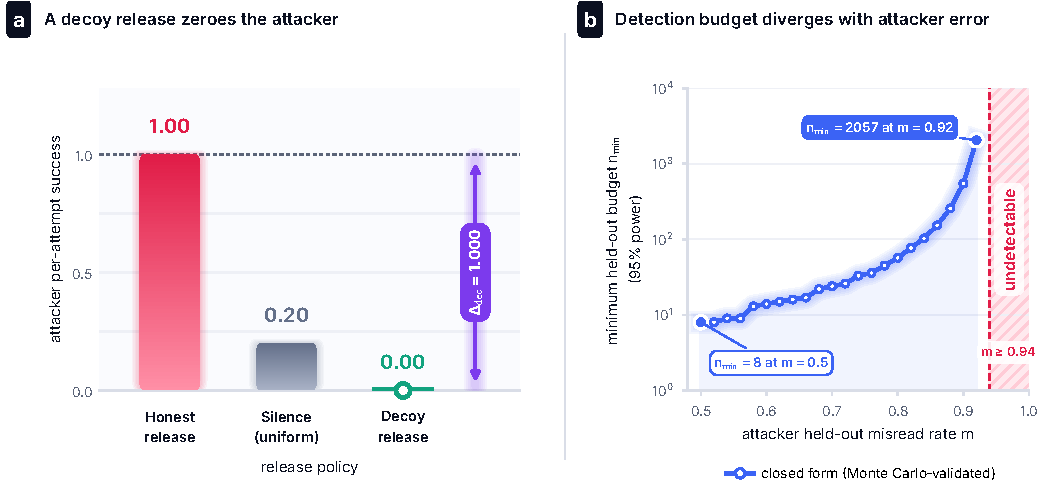
\includegraphics[width=\columnwidth]{anthro/fig5_premium.pdf}
\Description{Panel (a) plots attacker per-attempt success by release
policy: honest release at 1.0, decoy release at 0.0, silence at 0.2, with
the decoy collapsing monotonically toward the silence level as the
attacker's held-out verification capability grows. Panel (b) plots the
minimum held-out budget required for detection at 95\% power against the
attacker's probe-discrimination error on a log scale, diverging past a
few hundred at error rates above 0.9.}
\caption{The deception-release wave. (a)~E15: per-attempt attacker success
by release policy---decoy $0.000$ (stable under public verification),
honest $1.000$, silence $0.200$; the decoy edge collapses monotonically as
held-out capability arrives. (b)~E16: minimum held-out budget for
gaming-gap detection at 95\% power vs.\ discrimination error $m$
($m\ge0.5$ half of the grid); beyond $m\approx0.94$ no feasible budget
reaches the power, while any misclassification \emph{toward} the public
support fails the public certificate immediately.}
\label{fig:release}
\end{figure}
